\chapter{Getting started with Raspberry Pi}

\minitoc

\notesurl{intro1}

% TODO: Intro to what they have been given, and labelling their Pi
% TODO: References, references.
% TODO: Wikipedia links
% TODO: The Pi is yours to keep; if you lose it you'll have to buy another
% TODO: What you'll need to use the Pi at home
% TODO: Where do we introduce 'devices', 'files' and 'processes'? They will see virtual devices like tty0 and sda1 

\section{Introduction}

This and subsequent introductory labs contain a large amount of material. Don't worry if you can't complete it all during the timetabled lab session, but you should try to catch up outside the lab if you can. As always, if you're having problems, please tell someone and ask for help!

The Raspberry Pi is an astonishing piece of hardware. Not because it is super-fast or super-powerful---it's actually quite a slow computer by today's standards---but because it is small, cheap and needs very little energy to run. Its cheapness means you can experiment with it safe in the knowledge that if you mess it up, lose it, or drop it into the canal, getting hold of a replacement isn't going to cost you much more than a text-book or a night out at the cinema. Its small size and fairly modest power requirements mean you can be put to use in lots of applications where a regular-sized PC would be impractical.  We hope this will encourage you to experiment and explore, and to take risks playing with both its hardware and software that you might be reluctant to do on your own computer or tablet, or simply can't do with the School's lab machines. 

This lab session is designed to get you familiar with the Raspberry Pi itself, and with some of the basics of the Linux operating system it uses. We're going to be covering a lot of ground quite quickly, and it's important that you read these notes carefully and follow the instructions precisely for now. As the lab sessions progress, the instructions will become much less prescriptive, and we'll be encouraging you to experiment and explore much more, and to find out things for yourself. But for now, just follow our lead. 

\subsection{Breakout boxes}

Scattered throughout the main text of these exercises there are information boxes of various kinds:
\\

\begin{tabular}{m{1.5cm}m{12cm}}
{
\includegraphics[width=1.5cm]{images/bomb}} & \textbf{Danger!} The bomb icon explains problems and pitfalls, and how to avoid them. It's really important that you read these sections, or you may regret it later.\\
\\

\includegraphics[width=1.5cm]{images/rpi-logo} & \textbf{Raspberry Pi Facts and Factoids.} These sections explain useful but non-essential things about the Raspberry Pi. If you're pushed for time, you can safely skip these boxes and perhaps come back to them another time.\\
\\

\includegraphics[width=1.5cm]{images/diversion} & \textbf{We digress\ldots} Boxes marked with this icon contain digressions and facts that are hopefully interesting but are probably tangential to the main flow of the exercise.\\
\end{tabular}

\subsection{Styles and conventions}

We'll be using various typographic styles to indicate different things throughout these notes. When we introduce new concepts, or use terms that have a different meaning in computer science to their everyday use, they will appear \concept{like this}, and will be explained in the nearby text. Things that are either the input or output to commands will appear \ttout{in this font}. And many words or phrases will have a little `w' after them, meaning that if you click on the term (if you're reading the notes online) or type the phrase into \wikipedia{wikipedia}{Wikipedia} (if you're reading this on paper), you should be taken to a sensible definition in case you want to learn more about something that we've touched on here. 

Where you see text in square brackets [LIKE THIS] it will mean that when you're typing things you should replace the text with something that the text describes; for example [NAME OF THIS CITY], would become Manchester.

\FloatBarrier 
\section{The Raspberry Pi}

The most remarkable thing about the Pi is that, although it's not the most powerful of computers, it is capable of running the same full \wikipedia{Linux}{Linux} operating system as the machines that you'll be using in the labs for the duration of your studies, and which you'll undoubtedly encounter in your future careers. We're actually going to be using slightly different flavours of Linux on the Pi and the lab machines, but the differences are fairly minor---more on that later. Let's get started. 

The Raspberry Pi itself is just the circuit board shown from the top in Figure \ref{figure:bare-rpi}. The case we've put yours in is clear plastic so you can see the Pi inside, but you're welcome to change it for another style if you prefer (there are plenty available to buy online, and lots of people have made their own unique ones just for the fun of it). If you do put it in your own case, please remember to transfer the `sequence number' we've written on the underside of your Pi to the new box so that if the Pi is left behind in the lab it can be returned to you. The Pi is reasonably robust, and you can use it without a case, but obviously it's a bit more vulnerable if its not in a box of some sort. Figure \ref{figure:bare-rpi-underside} shows the Pi's circuit board from beneath, with an SD card inserted.

\begin{rpi}{Why Pi?}
  The Raspberry Pi apparently got its name because (a) lots of other computer systems have been named after fruit (you'll know of Apple and Blackberry, but in the past there has also been at least Apricot and Tangerine), and (b) the \wikipedia{Python_(programming_language)}{Python language} was one of the first things ported to run on it. The logo was created by Paul Beech, and is based on \wikipedia{Buckminsterfullerene}{Buckminsterfullerene}, a spherical fullerene molecule more commonly called a Buckyball. Its designer pointed out that a full buckyball has 32 faces, but that only 11 are visible in the 2D logo; and that the Raspberry Pi has a 32-bit processor and an ARM11 on board.

The ARM processor, on which the Pi and the vast majority of the world's other mobile devices are based, was originally designed by a team led by \wikipedia{Steve_Furber}{Steve Furber}, who is a Professor in this School.  
\end{rpi}

\subsection{Connecting the Pi}
\label{sec:connecting-pi}


\begin{figure}
\centerline{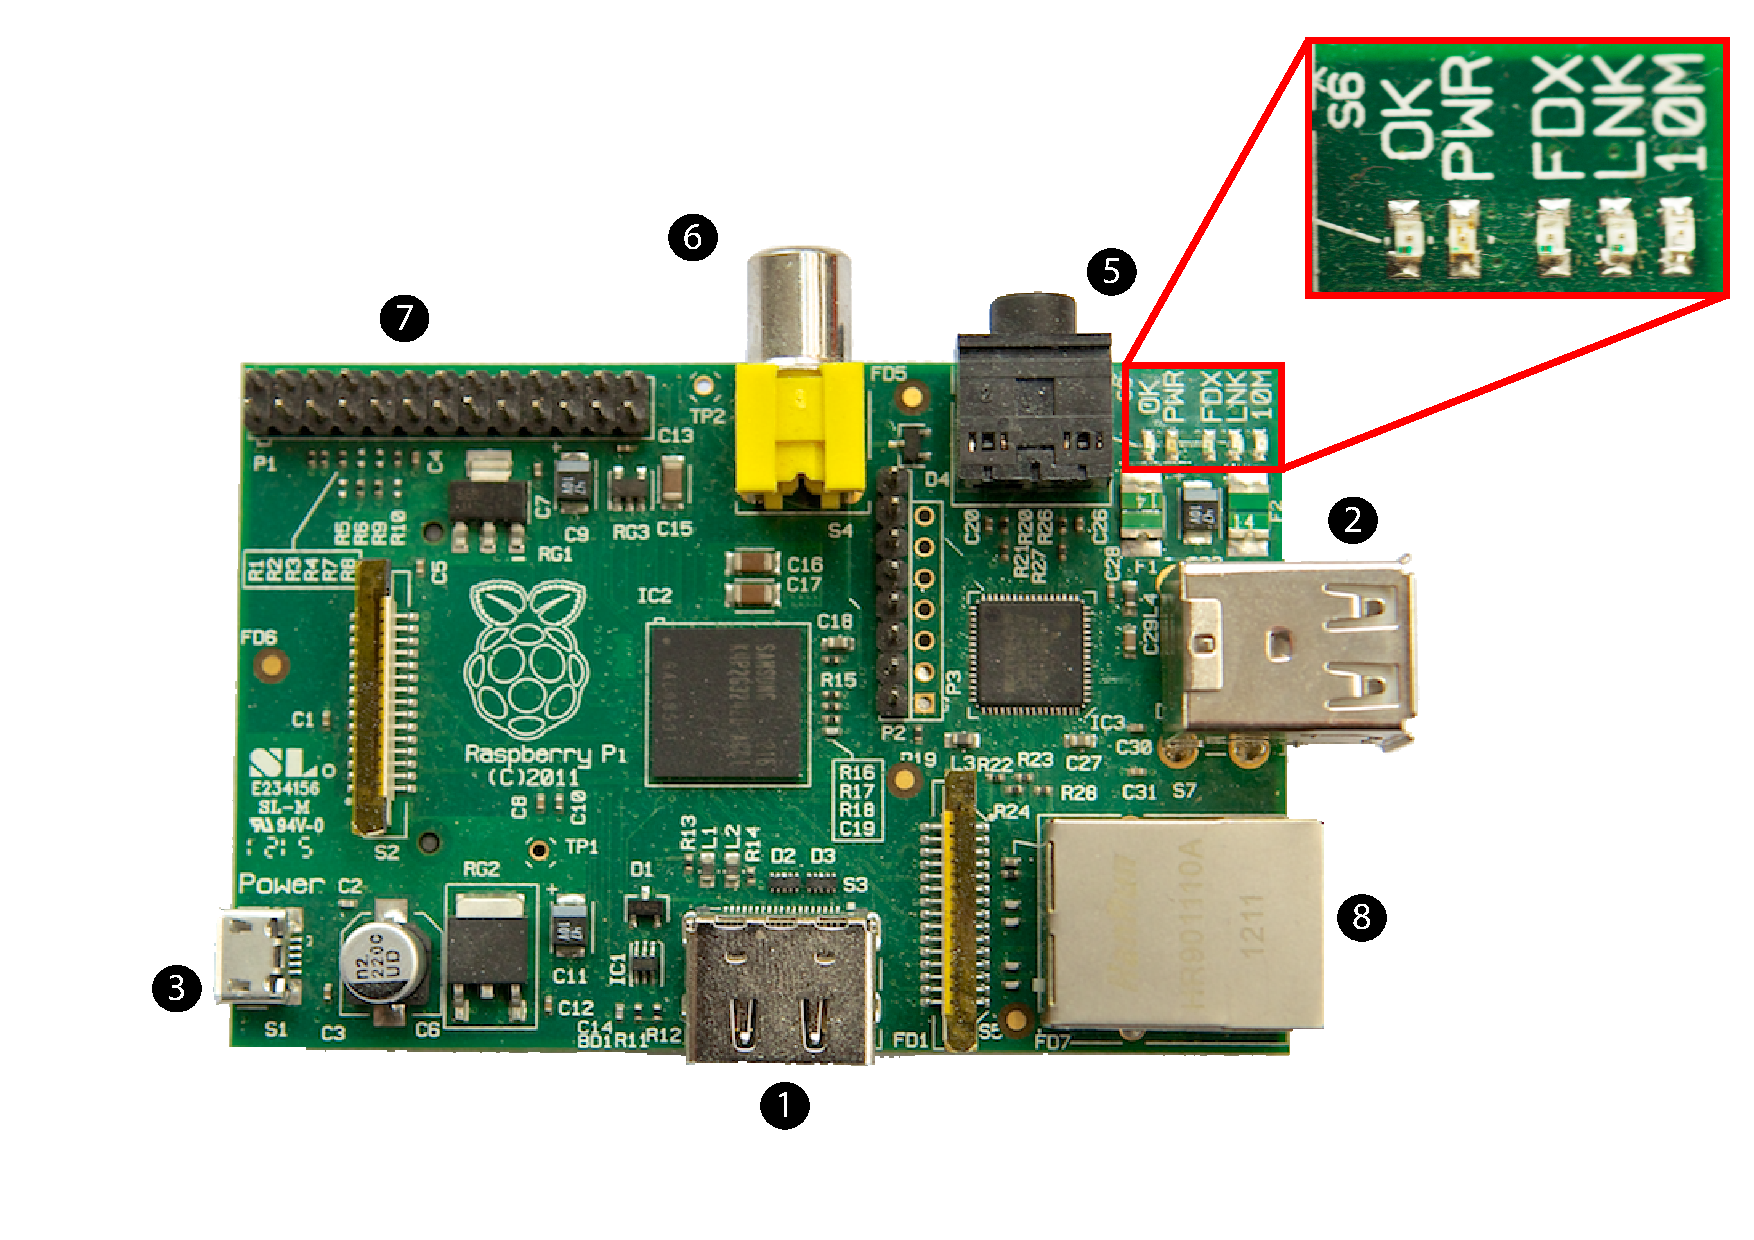
\includegraphics[width=15cm]{images/bare-rpi-annotated}}
\caption{An uncased Raspberry Pi, and an expanded view of the indicator LEDs at the board's top right. The numbered §connectors are \protect\circled{1} HDMI output,  \protect\circled{2} USB,  \protect\circled{3} power,  \protect\circled{5} audio output,  \protect\circled{6} composite video out,  \protect\circled{7} General Purpose Input/Output (GPIO),  \protect\circled{8} Ethernet.}\label{figure:bare-rpi}
\end{figure}

\begin{figure}
\centerline{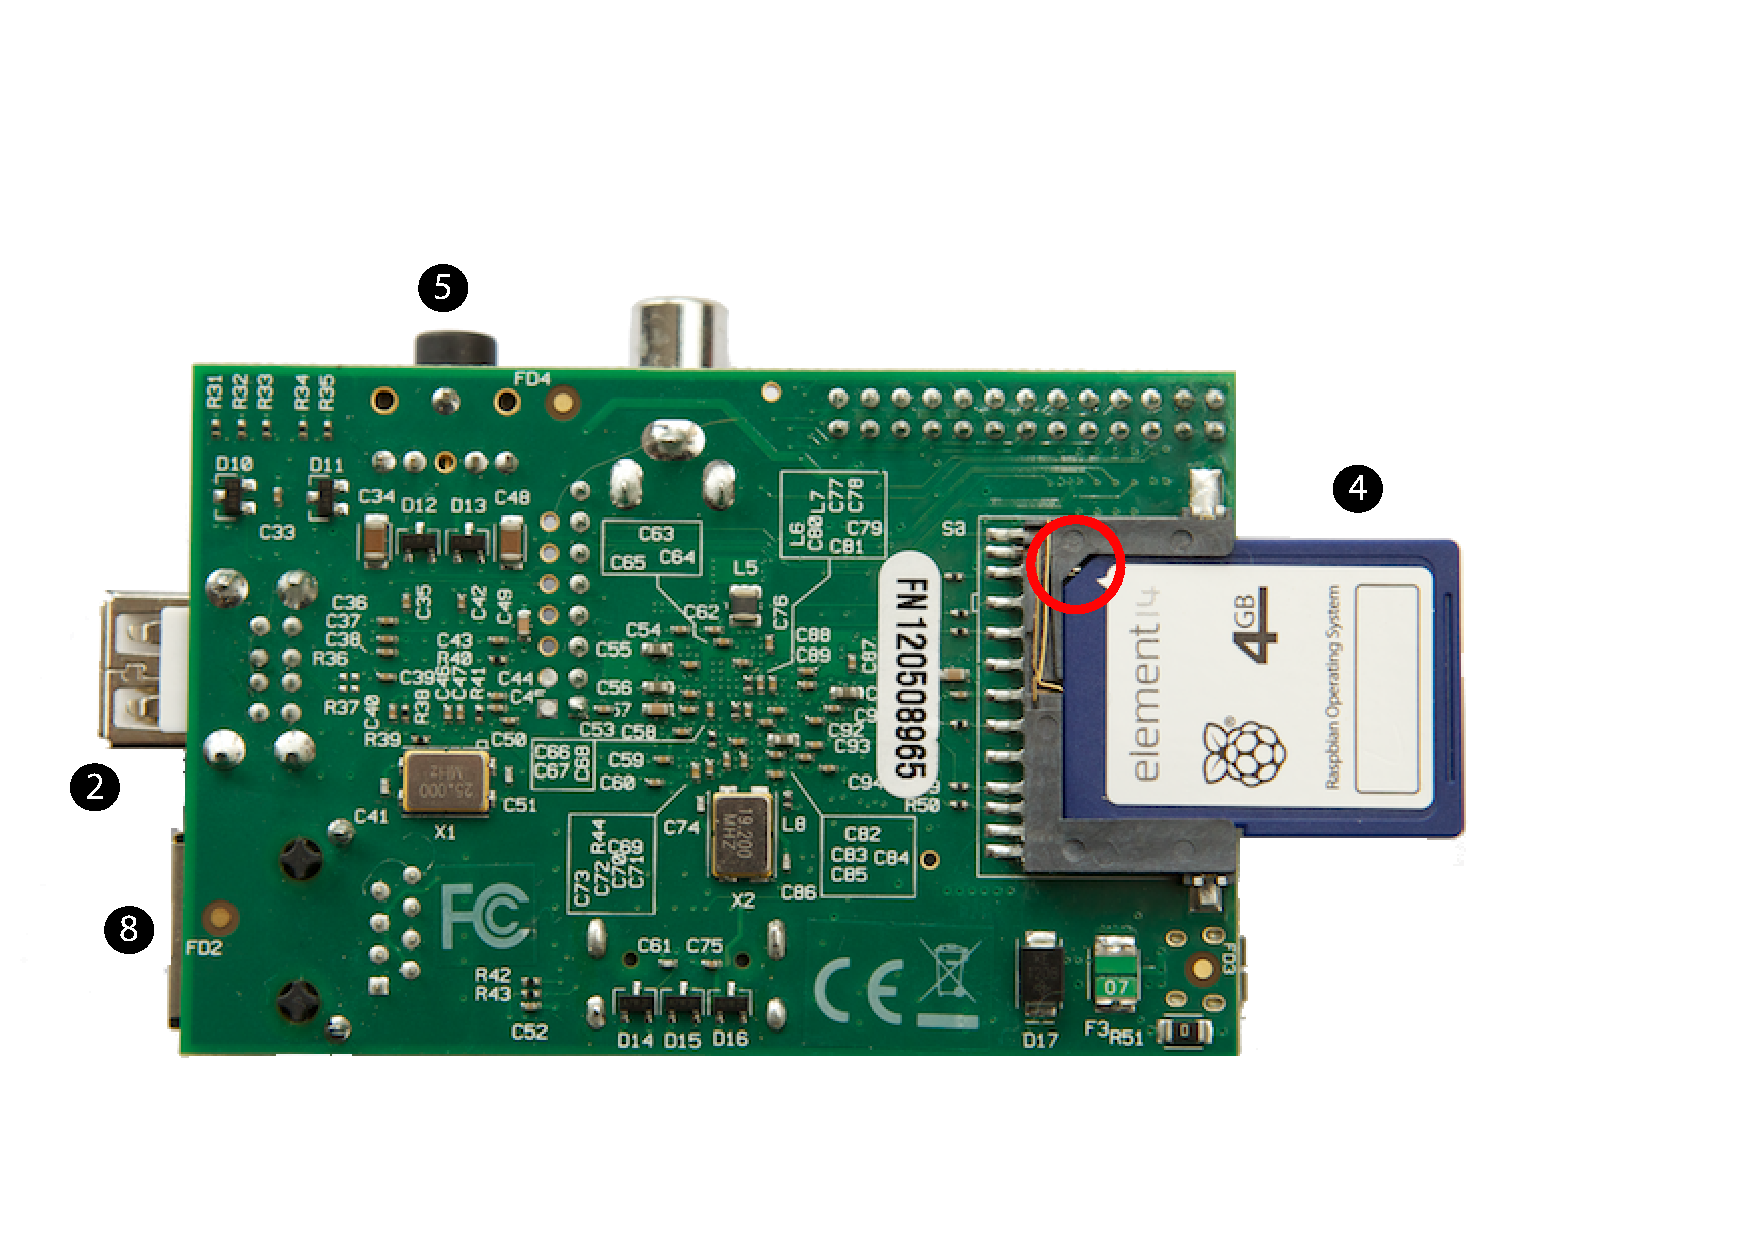
\includegraphics[width=15cm]{images/bare-rpi-underside-annotated}}
\caption{A naked Raspberry Pi. The circle indicates the location of the bevelled corner to orient the card. The ports are numbered as in Figure~\ref{figure:bare-rpi}, and in addition \protect\circled{4} shows the location of the SD (Secure Digital) memory card.  The locating bevel on the card is circled.}\label{figure:bare-rpi-underside}
\end{figure}

It's important that you connect the Pi up in exactly the order specified here---so even if you are familiar with using a Pi, please don't jump ahead and plug everything in at once (no harm will come to the Pi if you do, but this exercise relies on your following our instructions closely). Refer to Figure \ref{figure:cables}, and then connect your Pi up like this:

\begin{figure}
\centerline{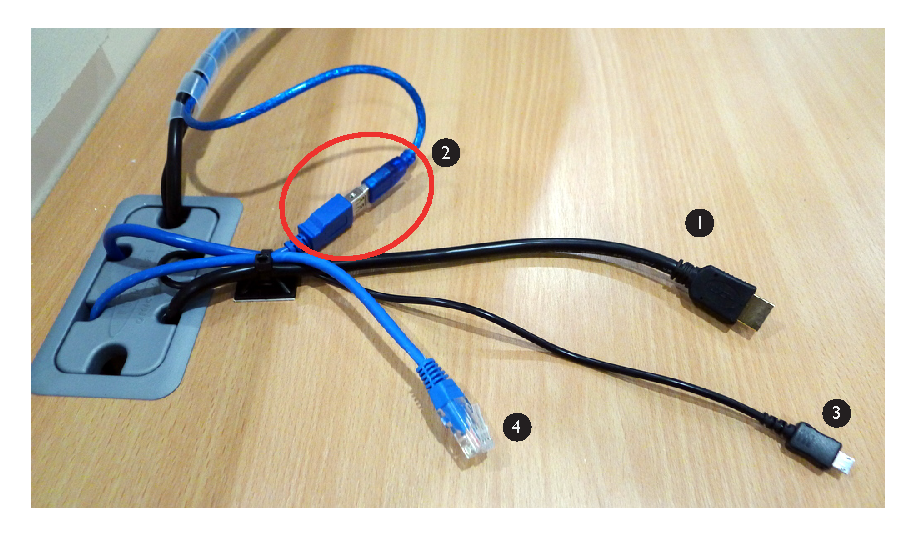
\includegraphics[width=13cm]{images/cables}}
\caption{The following cables are available to connect up your Pi. \protect\circled{1} HDMI, \protect\circled{2} Keyboard and Mouse, \protect\circled{3} 5 Volt Micro USB power supply, and \protect\circled{4} network.}\label{figure:cables}
\end{figure}


\begin{itemize}
\item The monitors in the LF31 Lab are all fitted with an extra video lead for connecting up the Pis. Locate the HDMI lead (labelled \protect\circled{1} in Figure \ref{figure:cables}), and plug this into the socket marked \circled{1} on Figure~\ref{figure:bare-rpi}. 
\item Next we'll need to connect a keyboard and mouse. Separate the male and female USB connectors marked \protect\circled{2} on Figure \ref{figure:cables}, and connect plug the male end into one of the two USB sockets on your Pi (marked with \protect\circled{2} on the Figure~\ref{figure:bare-pi}). It doesn't matter which USB socket you choose, but please make sure to reconnect this to the PC when you're done with these experiments as a courtesy to the next user. 
\item \textbf{Do not connect the power or network connectors at this stage!}
\end{itemize}

Next, we need to insert the \wikipedia{Secure_Digital}{Secure Digital} (SD) card that contains the Pi's operating system, and on which you'll be storing your own files. Look at Figure ~\ref{figure:bare-rpi-underside}, make sure the SD card is orientated correctly (note the position of the little cut corner) and gently push it into the socket; around half of the card will remain protruding outside the case. 



\begin{rpi}{Raspbian}
  The SD card we've provided for you has already had the standard Raspbian version of Linux written onto it (it's a version of the Debian release of Linux, tuned for the Pi). If you do manage to corrupt the operating system, or just want to start from scratch, then re-writing the SD card with a fresh image is reasonably straightforward: there are plenty of instructions online on how to do this, and we've provided you with a USB multi-card reader/writer that you can use for the job. The process does require access to what's called the `raw' device though, and on Linux that requires administrator access to the machine, so you'll have to use your home machine or someone else's Raspberry Pi to do this.

  Instructions on how to get hold of the files you'll need, and how to write them to the SD card on various operating systems are available at \urlnop{www.raspberrypi.org/downloads}. You might want to think about getting a larger SD card in any case; the one we've given you is fine for the labwork we've set, but probably a bit on the small side for anything else. SD cards are widely available in shops and online, and aren't expensive. But you should check whether the specific card you're going to buy is compatible with the Pi before parting with any money---differences in the read/write speeds of some cards mean they don't play nicely with the Pi.
\end{rpi}


Now you're ready to power up the Pi. In our lab setup in LF31 the power to the Pi is supplied via the monitor, so it is important that the monitor is not in standby mode. Standby is indicated by an orange light on the on/off button at the bottom right of the screen, rather than blue if it is on. If the light is orange, press it to turn the monitor off, then again to switch it back on and turn it blue. Now locate the 5v Micro USB cable (the same connector that you'll find on many modern smartphones and tablet devices); this is labelled \protect\circled{3} on Figure~\ref{figure:cables}. This goes into the socket marked \circled{3} on Figure \ref{figure:bare-rpi}. There is no power switch on the Pi, so as soon as the power cable goes in, it will start to boot (this strange term is explained in breakout box~\ref{bootbox}): the red PWR LED should light up and stay on, and you'll also notice that the OK LED (which indicates SD-card activity) to its left also flickers. If any of the other three LEDs marked FDX, LNK, or 10M are lit, then that means you've already plugged a network cable into your Pi, in which case please unplug that now!

\begin{danger}{Pi Power} 
Like most other computers, the Pi doesn't like having its power removed without being shut down properly. Although you might get away with it, there's a reasonable chance of messing up the operating system if you remove the power while the Pi is in the middle of doing something. And because the Pi runs a multi-tasking operating system, it's almost always `doing something', so pulling the power out unexpectedly is always a bad idea. You're unlikely to damage the Pi's hardware like this, but you may find that you lose work, and may have to reinstall the operating system. For instructions on how to shut the Pi down safely, see Section \ref{section:shutdown}.
\end{danger}

Now we need to switch the input on the monitor from DisplayPort (which
is the input used by the PC under the desk) to DVI (the cable you've
connected your Pi to is a HDMI to DVI cable). On the lower-right side
of the monitor you will see 4 buttons -- see
Figure~\ref{figure:monitorswitch}. Press any of them to bring up the
monitor's menu. Now press the 3rd button down and navigate to the
input selection menu. Switch the Input to DVI and all being well you
should see a black screen containing the Raspberry Pi logo at the top
left, and white text that scrolls up the screen as the Pi boots. When
the boot process finishes for the first time (it will take somewhere
about 20--30 seconds), if all has gone well you should see the Pi's
configuration tool appear (see Figure \ref{figure:raspi-config}).

% TODO: needs a photo of the monitor / switch here
\begin{figure}
\centerline{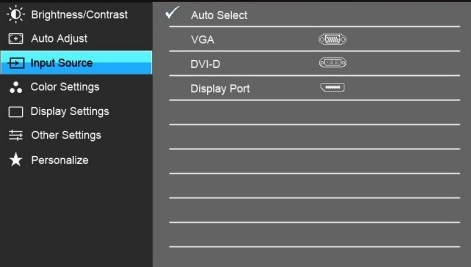
\includegraphics[width=12cm]{images/DellInputMenu.jpg}}
\caption{The Input Selection menu on the monitor. This image  of the Dell U2412M Monitor has been reproduced with the kind permission of Dell. All rights reserved.}\label{figure:monitorswitch}
\end{figure}

\begin{diversion}{Booting}
\label{bootbox}
The phrase `booting' to refer to the process of starting up some computer system has become quite commonplace, but its origins are rather strange. It's thought to have first been used in early 19th Century America as a way of describing an obviously impossible action such as to ``pull oneself over a fence by one's bootstraps''. These days it is used to refer to any self-sustaining process that is able to happen without external help. 

So why is starting a computer a bootstrapping process? In order for you as a user to be able to run a program, the computer needs an operating system. But in order to load its operating system, it needs some instructions that tell it how to understand the file system. And in order to load the instructions that tell it how to understand the file system it needs to\ldots well, you get the idea. In reality, most computers have a very small set of instructions hardwired into them that begin the process of loading a  slightly more complex `bootloader', which then begins the process of loading the OS kernel and any modules needed to interact with the hardware, and then starts loading services and features of increasing sophistication that rely on the simpler ones loaded previously to function. 

As an aside, you may want to consider this: if you need a text editor to write programs, how did the first text editor (which is itself a program) get written?
\end{diversion}

\begin{figure}
\centerline{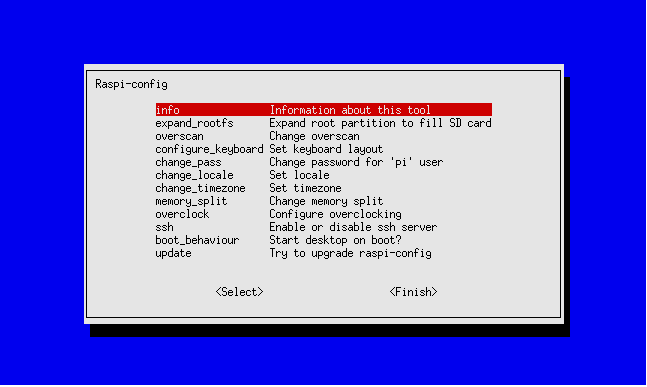
\includegraphics[width=13cm]{images/raspi-config.png}}
\caption{The Raspberry Pi config tool. The highlight bar can be moved between the different controls using the Tab key, or up and down in the menu using cursor keys.}\label{figure:raspi-config}
\end{figure}

Before using the Pi for real, you'll need to perform one task using this menu. Use the up and down cursor keys to move the selection bar to the \ttout{expand\_rootfs} option, and press Enter. You'll see a confirmation that `Root partition has been resized. The \wikipedia{File_system}{filesystem} will be enlarged upon the next reboot'. If that doesn't mean anything much to you right now, don't worry, we'll come back to an explanation of that later. For now just press Enter again to get back to the main menu. 

At this stage you could tweak various other options that affect the
display and the layout of keyboard being used; but conveniently the
defaults set on the Pi will do just fine for now (it is a mostly
British invention after all, so it defaults to UK keyboard layout!)
Use the Tab key to move the red highlight to \ttout{<Finish>}, and hit
Enter again. Confirm that the Pi should reboot (an example of what
this looks like is shown in Figure \ref{figure:piboot}) and this time
when the process finishes you'll be presented by a Unix login prompt
which will say something like:

\begin{figure}
\centerline{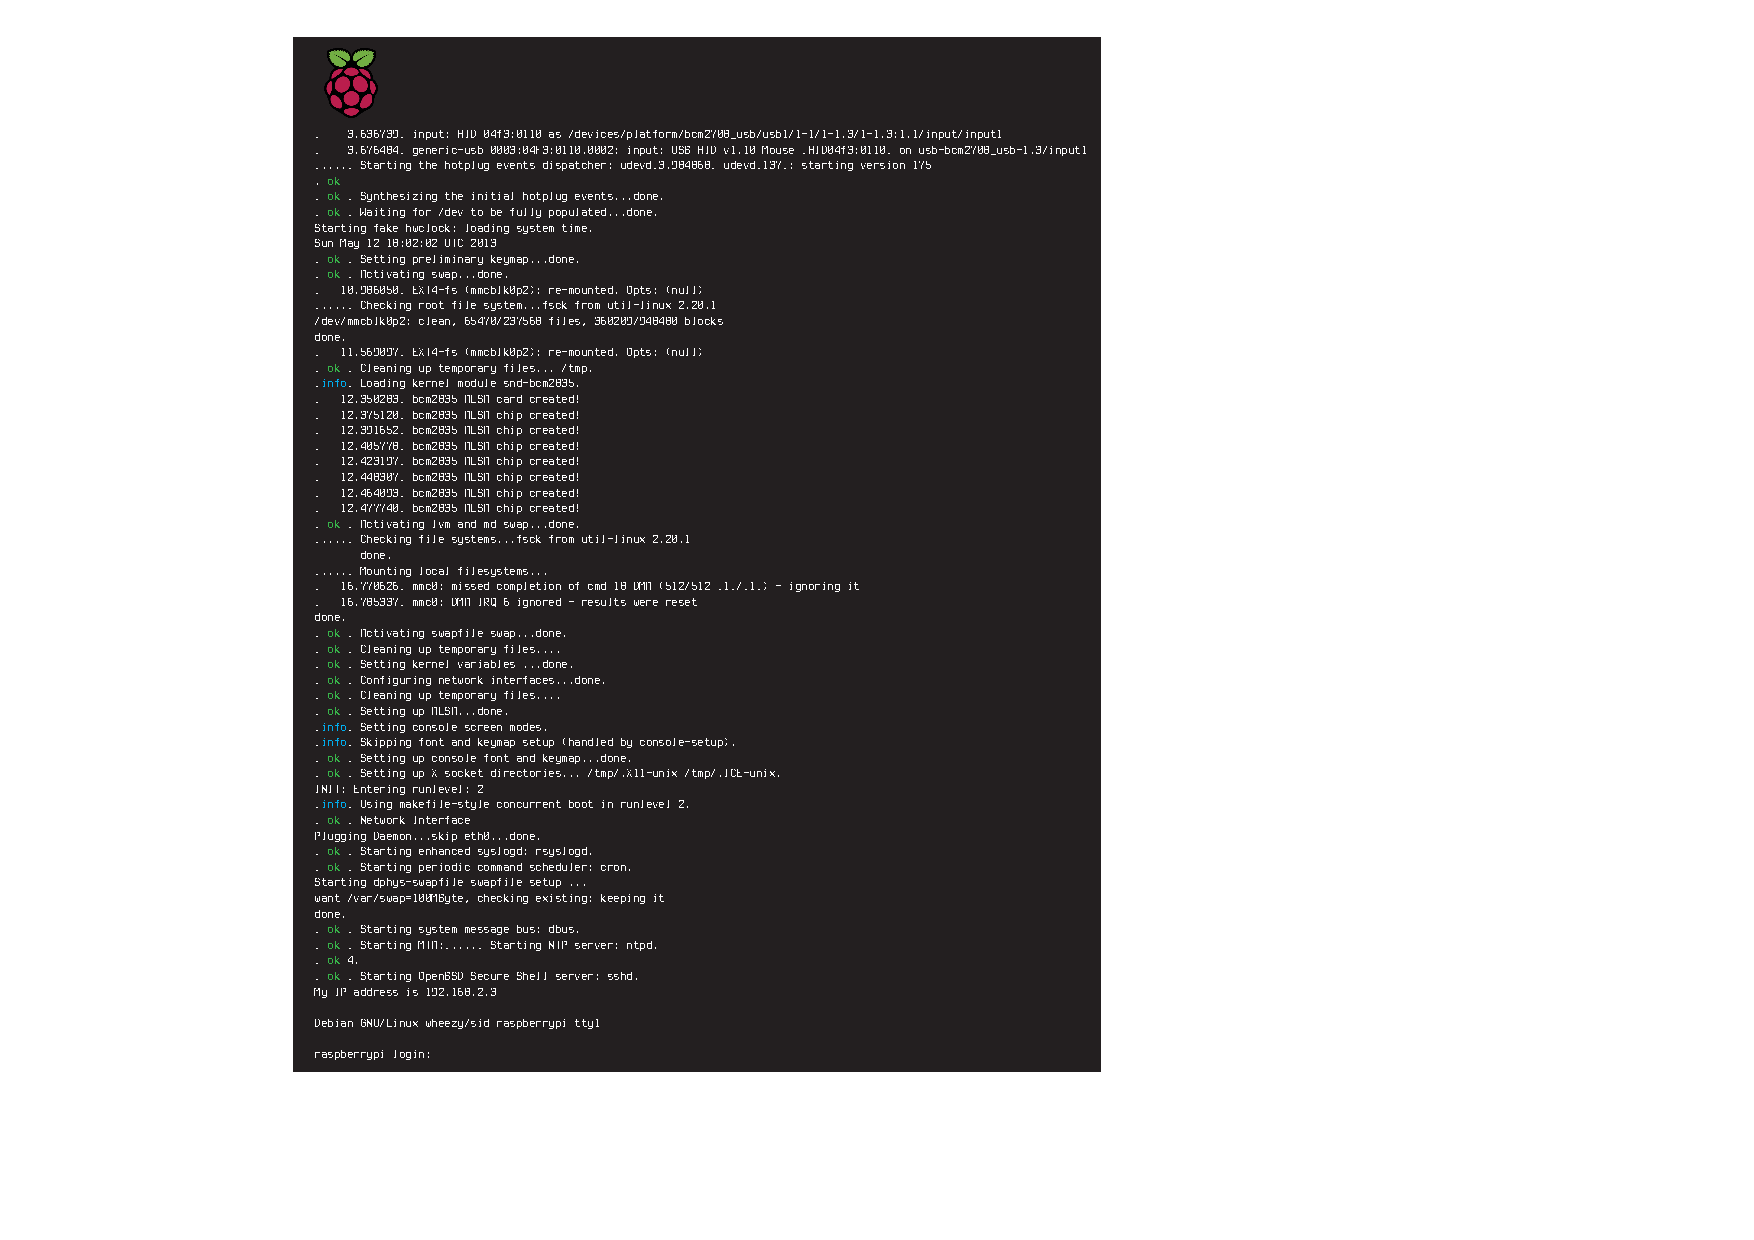
\includegraphics[width=15cm]{images/bootscreen}}
\caption{A sample Raspberry Pi bootscreen. The exact layout and details may vary depending on the size/shape of the screen and the configuration of the Pi.}\label{figure:piboot}
\end{figure}

\begin{ttoutenv}
Debian GNU/Linux wheezy/sid raspberrypi tty1

raspberrypi login:
\end{ttoutenv}

\subsection{Using the Pi}
\label{sec:using-pi}

At the login line enter \totype{pi} as the username, and when prompted for the password, type \totype{raspberry}. \textbf{Note that, so that anyone standing behind you cannot even see the length of your password,  the username will appear on screen as you type it, but the password will not} (so make sure you're typing carefully!) You should see:

\lstset{moredelim=[is][\textbf]{|}{|}}
\begin{lstlisting}
Last login: Mon Feb 16 14:46:27 2015
Linux raspberrypi 3.18.7-v7+ #755 SMP PREEMPT Thu Feb 12 17:20:48 GMT 2015 armv7l

The programs included with the Debian GNU/Linux system are free software;
the exact distribution terms for each program are described in the
individual files in /usr/share/doc/*/copyright.

Debian GNU/Linux comes with ABSOLUTELY NO WARRANTY, to the extent
permitted by applicable law.
|pi@raspberrypi ~ $|
\end{lstlisting}


%

The last line of this text (which is shown in bold here but will be green and blue on your screen) is the \wikipedia{Command_Prompt}{command prompt}. It might look innocent enough, but in the right hands, the command prompt is one of the most powerful ways of controlling a computer. Your previous interaction with a computer was probably via  a \wikipedia{Graphical_User_Interface}{graphical user interface}, or GUI, such as that provided by Windows or Mac OS X, so  it may feel a bit odd at first to be issuing instructions to a machine via a textual command-line. However, this is a crucial skill that you'll need during your studies here at University, and also in your future career. In fact, employers have often said that our students' abilities with the command line come as a very pleasant surprise to them.


\begin{diversion}{Don't be a WIMP}
\label{breakout:wimp}
The familiar Windows, Icons, Menus and Pointer (WIMP) paradigm used on most graphical desktop environments is enormously powerful, but it's not suitable for every task, and understanding when you're better off using the command-line or a keyboard shortcut instead will make you a lot more efficient.

Sometimes the clumsiness of the GUI comes from the fact that there's no convenient visual metaphor for a particular action; how do you graphically represent the concept of `rename all the files I created yesterday so they start with a capital letter'? 

But a lot of the time the issue is simply that it takes much longer to do some things with the mouse than it does with a keystroke or two. Every time you use the mouse, a little time is wasted shifting your hand off the keyboard and a little more time used up tracking the pointer between the on-screen widgets. For casual use, this wasted time really doesn't matter. But as a computer scientist you're going to be spending a lot of time time in front of a machine, and all the seconds wasted moving the mouse pointer around add up. 

What's really fascinating here, though, is that although the keyboard versus mouse debate is one that has been running for at least the mid-1980s, there isn't a clear winner, or even any definitive guidelines as to when one is better than the other. 

In any case, you should definitely learn the keyboard shortcuts for the most common operations in your favourite tools, and a handful of useful command-line tools. For example, when you're writing code you'll be saving files very regularly; maybe even several times a minute when you're debugging. There are two options for this: 1) move hand off keyboard to mouse; use pointer to find the `File' menu, from the file menu move the pointer to the `Save' option; move hand from mouse back to keyboard. Or 2) Press the combination of keys that perform the `save' function. Which do you think is faster?

And think carefully about the best tool for the job; sometimes it'll be the mouse/menu combination, but perhaps more often than you might think, a few selected commands may get the job done considerably more quickly. In particular, you've probably had more experience of doing things the GUI-way up until now, so if it's not obvious which is the better choice for a particular task, we suggest you go for the command-line option until you're familiar enough with the pros and cons of both approaches to make an informed decision each time.
\end{diversion}

The default command prompt on the Pi consists of four components shown in Figure \ref{figure:prompt}.

\begin{figure}
\centerline{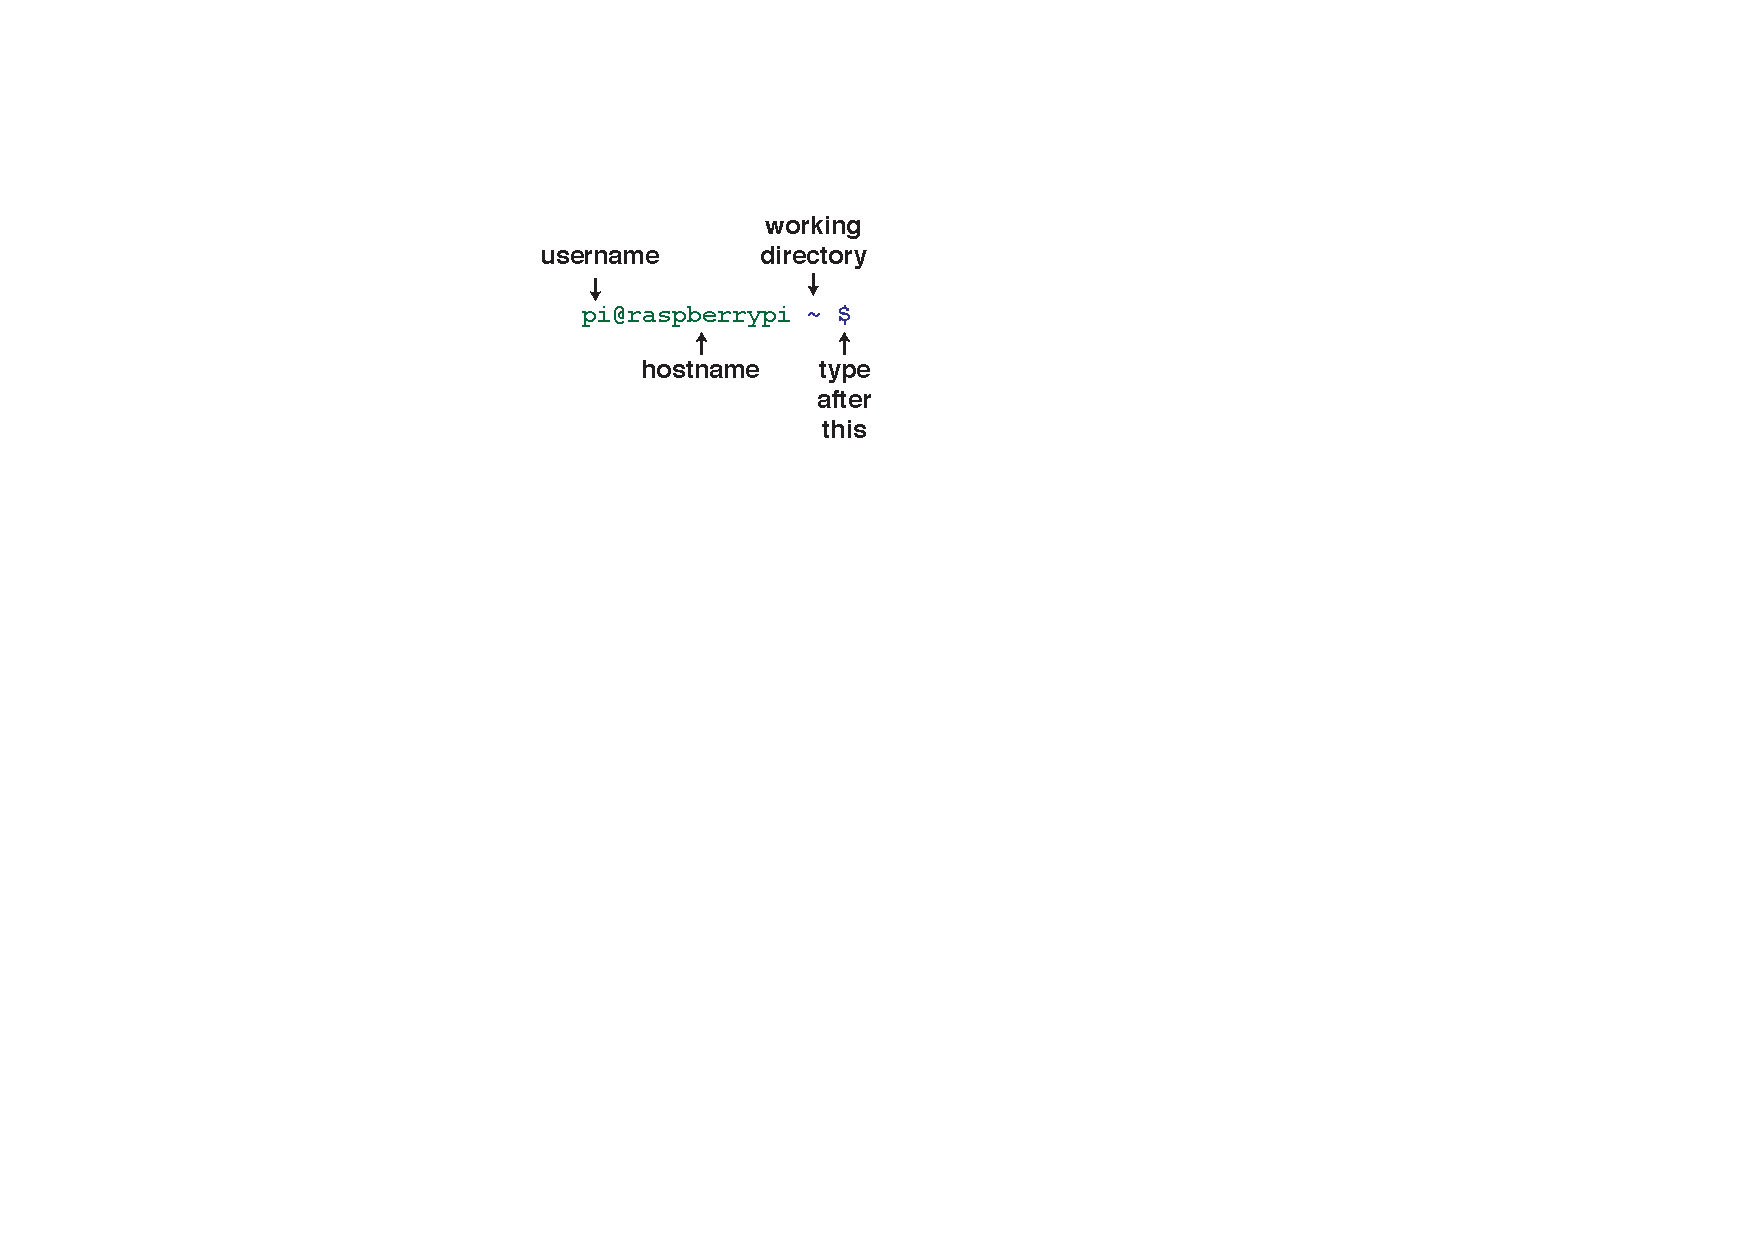
\includegraphics[width=7cm]{images/default-prompt}}
\caption{The different components of the Pi's default command prompt.}\label{figure:prompt}
\end{figure}


\begin{itemize}
\item To the left of the \ttout{@} symbol is the name of the user, and in this case that's \ttout{pi}, since you've just logged in under that name
\item To the right of the \ttout{@} is the hostname of the machine, which on a Raspberry Pi is quite reasonably set to \ttout{raspberrypi} by default.
\item The \texttildelow{} tells you where in the Pi's file system you're currently working. We'll explain this in a lot more detail later on, for now all you need to know is that the \texttildelow{} symbol is called a \textit{tilde} (pronounced something like till-duh, though it's often referred to colloquially just as a `twiddle'), and is used here to refer to the `home' of the current user. 
\item On the Pi the default prompt ends with the \$ symbol. 
\end{itemize}

You can change this prompt to something more or less verbose later, but for now we'll leave it as it is. For simplicity in these notes, we'll use the \$ symbol from now on to mean `type something at the command prompt and press Enter'. So for example

\begin{ttoutenv}
$ echo Hello World
\end{ttoutenv}

\noindent means `type \totype{echo Hello World} at the command prompt and then press Enter' (you can do this if you like; the result will be that `Hello World' gets `echoed' \cmnd{echo}{} back to you on the next line of the screen). (Notice that this reference to a Unix command has caused a small cog to appear in the right hand margin, so you can find this reference easily later. If you are reading the notes online, the cog also contains a link to a web page describing some unix commands)

Before we do any real work on the Pi, we should make it a bit more secure than it currently is. Remember, you've logged in using the default username `pi' and the default password `raspberry', so anybody else could do the same; so this is the time to change the password to something that's unique. 

For webcomic XKCD's view on creating good passwords, see Figure \ref{figure:xkcd-password}.

\begin{figure}
\centerline{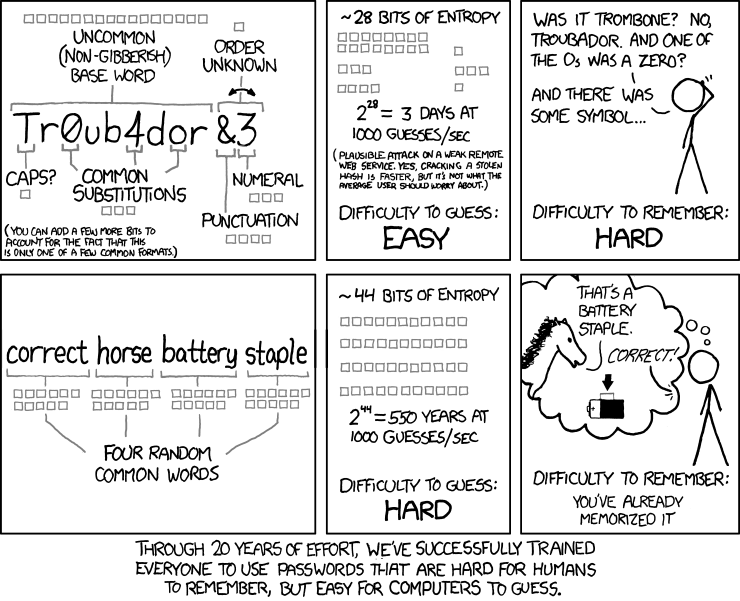
\includegraphics[width=13.5cm]{images/xkcd-password-strength}}
\caption{XKCD's take on password creation \urlnop{xkcd.com/936/}}\label{figure:xkcd-password}
\end{figure}

The command to change the password on the Pi is \cmnd{passwd}{passwd}; typing this at the command prompt and entering your current password (i.e. `raspberry') and new password (twice, to be sure), should look like this:

\begin{ttoutenv}
$ passwd
Changing password for pi.
(current) Unix password:
Enter new Unix password:
Retype new Unix password:
\end{ttoutenv}


\noindent Note in the above, we're using lines that don't start with the dollar symbol to show output as a result of what you've typed, and that none of the passwords you're typing actually appear on screen for obvious sneaky over-the-shoulder-peeking reasons. \textbf{Don't forget this password: there's no easy way to get back into your Pi without resetting everything.}

Are you sure you know what your password is? If so then type \cmnd{logout}{logout} at the command prompt. Not surprisingly this will log you out of your Pi. Then log back in again using your new password. 

\begin{danger}{Memory Loss} 
Although the Pi uses a fairly standard Unix operating system, it's probably not quite as secure as a normal desktop machine because of its small size and easily-removable storage media. Once the Pi has booted from the SD card, it's about as secure as any other Linux machine. But because the memory card is easily removable, it can trivially be connected to another machine as a `removable media' device; and at that point the host machine can almost certainly see its contents, including any of the files you've created, because the filesystem itself isn't encrypted. And because the Pi is small and portable, it's easier to lose it than a laptop or desktop machine; so, be careful!
\end{danger}

Now that your password isn't the same as the `out of the box' Pi one, it's safe to plug your Pi into the network. Locate the blue ethernet cable poking out of the desk (labelled \protect\circled{4} on Figure~\ref{figure:cables}); plug that into the appropriate socket on your Pi (number \circled{8} on Figure~\ref{figure:bare-rpi}) and you should see the FDX, LNK and 10M LEDs light up. To confirm that you're now connected to the network, use the \cmnd{ping}{ping} command, which sends a low-level network message to a designated place and checks for a response, to see if you can reach our School's web server. 

\begin{ttoutenv} 
$ ping www.cs.manchester.ac.uk
PING waldorf.cs.manchester.ac.uk (130.88.194.191): 56 data bytes
64 bytes from 130.88.194.191: icmp_seq=0 ttl=52 time=37.914 ms
64 bytes from 130.88.194.191: icmp_seq=1 ttl=52 time=40.392 ms
64 bytes from 130.88.194.191: icmp_seq=2 ttl=52 time=41.006 ms
\end{ttoutenv}

% $

Each of the lines starting with `\ttout{64 bytes}' represents a short response from the machine you've just pinged, and you're shown the round-trip time for ping's data to leave your Pi, find (in this case) \url{www.cs.manchester.ac.uk} on the network, and return back to your Pi. Since we're just using ping here to give us some confidence that the network is okay, we don't need to leave it pinging away for ages, so let's stop the ping command in its tracks. Hold down the control key (marked `ctrl' on the keyboard), and press `c'. This will signal the currently executing command that it should stop what its doing and return to the command prompt (quite often this is referred to as ``control-c'ing'' a command, and it will have the same effect on the majority of command-line tools). This process is often written \ctrl{c}. \textbf{If you see this notation in these notes, don't type the individual characters, press the key marked ctrl and the appropriate letter key}. 

\begin{diversion}{Ping}
  The \ttout{ping} command is named after its use in the field of active sonar, where an actual `ping' sound was sent through water, and distance calculated by listening for the echo to return. It's the classic boingy pingy noise associated with submarine movies! 
\end{diversion}

\section{Processes and the Unix Shell}

Before doing anything else, let's take a few steps back and look in a bit more detail at what you've just done; you may be surprised how much stuff happened as a result of that simple command you've just typed. 

The first concept you'll need to understand is that you have been
interacting with what is known in Unix circles as a \wikipedia{Shell_(computing)}{shell}: a program that prompts
the user for commands, accepts them, executes them and displays the
results. A shell is just a program running on the Linux operating system like any other program---it's not `built in' to the computer or the operating system in any special way, it just happens that by default, the Pi is set up so that when a user logs in, the first program that gets executed on behalf of that user is an interactive shell that allows users to execute further programs themselves. Later in your degree programme you'll look at the file that determines which program gets executed first for a user, and indeed at the order in which programs are run by the operating system as it boots up, because in Linux all of these things can be easily configured by changing a few lines in the appropriate text file. For now, it's enough to understand that the shell is just a program that interacts with the user via the keyboard and display, and allows you to execute commands to do useful things.

But what do we mean by `execute commands'? And if the shell is `just a program', how does it get to communicate with the keyboard and monitor? What is a `command' anyway, where do commands come from?

To understand what's going on here you'll need to make sense of a concept that's fundamental to pretty-much any operating system; that of a \wikipedia{Process_(computing)}{process}. As you no-doubt know, modern computers have one or more \wikipedia{Central_processing_unit}{Central Processing Units} (CPUs) which are capable of carrying out simple instructions; a basic computer like your Pi will have a single CPU, whereas a big server machine or supercomputer may have several tens of CPUs in a single box. To a first approximation, each CPU is only capable of following one instruction at a time, and the illusion that a computer is capable of doing a very large number of things simultaneously (e.g. streaming music, displaying web pages, downloading a video of a unicycling kitten and playing \wikipedia{Minecraft}{Minecraft}) is achieved by the operating system arranging for each of these tasks to be given access in turn to the CPU for a tiny fraction of a second. More technically, the unit of activity that's being scheduled to run on the CPU is called a \wikipedia{Process_(computing)}{process}. The relationship between anything that you as a user may recognise---for example a desktop application---and what's happening in the operating system in terms of processes is quite complex, since many applications are made up of several processes, and there will be a whole load of other processes doing housekeeping jobs that aren't immediately obvious to a user. But for now we'll gloss over this detail and work on the assumption that when you ask a computer to do something for you, a process will be started to deal with that task for you. 

\begin{figure}
\centerline{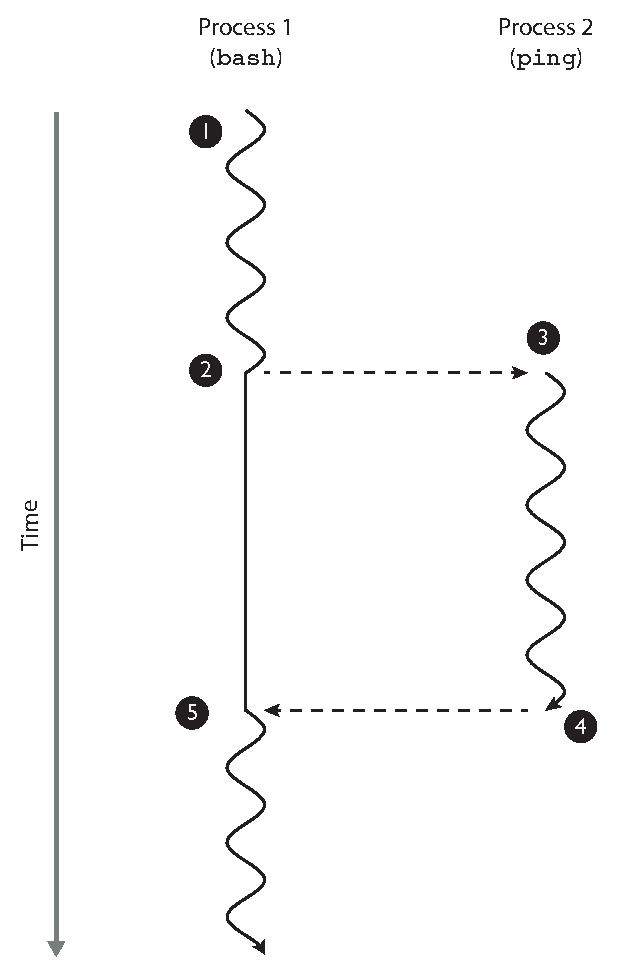
\includegraphics[width=7cm]{images/bashandping}}
\caption{Running a command at a bash shell involves two process, one for the bash shell itself, and a second child process that is started by the bash shell in which to run the command: \protect\circled{1} initially, just the bash process is running. \protect\circled{2} at the point where you type the ping command and press enter, bash starts a second process and hands over its input and output to that new process, which executes the command on your behalf; at this point the bash process continues to exist but `goes to sleep' until the command finishes. \protect\circled{3} the new process starts up, and executes your command, until at \protect\circled{4} it's either aborted by the user or finishes what it's doing, at which point \protect\circled{5} the ping process terminates and hands back control to the shell, which wakes up ready to accept the next command.}\label{figure:bashandping}
\label{fig:bashandping}
\end{figure}

In terms of what's just happened when you ran the \cmnd{ping}{ping} command a
moment ago, there are at least two processes involved. The shell
program itself is a process that's waiting for you to type something
at the keyboard; when you pressed enter after having typed your
command, the shell interpreted your input, and started up a second
process to run the \cmnd{ping}{ping} program for you. It handed 
access to the keyboard and monitor over to the process running \cmnd{ping}{ping},
and then then went to sleep briefly to wait for the \cmnd{ping}{ping} command to
finish. When \cmnd{ping}{ping} finished (in this case because you aborted it), the
shell woke up again, took back control of the keyboard/screen, and was
ready for your next instruction. This is illustrated in Figure
\ref{fig:bashandping}.

You will learn much more about processes and the way they are managed in COMP15111 and COMP25111; for now there's one more thing you need to understand about the relationship between processes. 

\subsection{The process `family tree'}
\label{section:family-tree}

When the shell's started up a process to run your command, the new process (the one that's running the command) is thought of as a `child' of the shell's process. The child inherits many of the properties of its parent (you'll see why this is important in the next Pi lab), generally speaking the child cannot exist without its parent. If something caused the parent process to abort, then the child process would also die. If the child process for whatever reason itself starts up any new processes, they would be its children (and, if you like `grandchildren' of the original shell); so in this case, causing the shell to die would wipe out all its offspring. Generally this is the behaviour that you want (it certainly is for most commands issued from the shell), but some times you want a process that you've started to outlive its parent (for example, to continue running even when you've quit your shell and logged out). We'll look at this behaviour in much more detail later in the course.


\begin{diversion}{Unix shells}
Unix has many shells: the first shell was called the `Thompson' shell (also known as just `sh', and pronounced ``shell''), written by Ken Thompson for the first Unix system; then came the `Bourne' shell (also called `sh'), written for a later commercial version of Unix by Stephen Bourne. You have just been using the Free Software Foundation's `Bourne Again' shell (a pun-name taking a dig at its commercial fore-runner), or `bash'. The various different shells offer the user different facilities: `sh' is rather
primitive compared to the more modern ones. However, their basic
functionality is always the same: they accept commands from the
\concept{standard input} (for now, we can treat that as meaning `the keyboard'), execute them, and display
the results on the \concept{standard output} (i.e. for now `the screen', which in
this case was the entire screen, or \textbf{console}). Shells repeat
this process until they have reached the end of their input, and then
they die. Unix shells are rather like \textbf{Command Prompt} windows in Microsoft
Windows, except that Unix shells are considerably more sophisticated.
\end{diversion}



\section{Files systems and files}

Next we're going to explore the Pi's filesystem a little. You'll be familiar with the idea of a hierarchy of files and folders from whatever graphical environment you're used to using on desktop or mobile devices: files represents things that you've created or downloaded such as documents, images or movies, and folders are a way of organising these into related collections. By putting folders inside folders, you can organise your stuff starting with general concepts such as `Photographs' and ending up with much more specific collections, e.g. `Holidays', then `Bognor Regis 2013'. 

Interacting with a standard Unix filesystem via the command-line uses similar concepts (actually, it's the graphical environment that's being `similar' here really, since the Unix command-line existed quite some time before anything graphical appeared). Files are called files, but what are commonly represented as `folders' in graphical environments are more correctly called `directories' when we are operating at this level (and we'll call them directories from now on, because it'll make some of the command names and manual pages make more sense). 

Let's first see what stuff we already have on our Pi. The \cmnd{ls}{ls} command lists files and directories. Type it now, and you should see that two folders have already been created for you, one called \fname{python\_games} and the other called \fname{Desktop}. 

\begin{ttoutenv}
$ ls
Desktop python_games
\end{ttoutenv}

% $

When we're using a command-line prompt, we have the notion of of \wikipedia{http://en.wikipedia.org/wiki/Working_directory}{current working directory} which is the directory that we're currently `in' (so in this example, using \totype{ls} like this really meant `run the list command on my current working directory'.) There are numerous Unix commands that allow you to move around the filesystem's directory structure, and it's very important that you become familiar with these early on. 

Let's say we want to look at the contents of the \fname{python\_games} directory. There are several ways of doing this, but for now we'll break the process down into simple steps. Use the \cmnd{cd}{cd} command to Change Directory to \fname{python\_games}:

\begin{ttoutenv}
$ cd python_games
\end{ttoutenv}

and look at what's happened to the command prompt. Whereas before it was just
\\
\\
\totype{pi@raspberrypi \texttildelow{} \$}
\\
\\
it has now become
\\
\\
\totype{pi@raspberrypi \texttildelow{}/python\_games \$}
\\
\\
to indicate that we've changed our current directory to \fname{python\_games} (remember the \texttildelow{} symbol means `home directory', so \fname{\texttildelow{}/python\_games} really means 'a subdirectory called \fname{python\_games} which is in my home directory').

Now use the \cmnd{ls}{ls} command to list the contents of our new current working directory. You should see a long list of files: some are programs written in the Python programming language (these files end in \fname{.py}), others are images or sounds used by those programs (ending in \fname{.png} or \fname{.wav}). At the prompt type:

\begin{ttoutenv}
$ python wormy.py
\end{ttoutenv}

to start a simple version of the classic `Snake' game. You can guide your green snake around the screen with the cursor keys; you score a point every time you eat one of the red squares and an extra segment gets added to the length of your snake. The game finishes if you crash into the edge of the screen or eat yourself. Once you've convinced yourself this is working (don't spend too long playing the game!), press the Escape key to return to the command prompt. You'll be writing a more sophisticated version of this game soon enough in the Java labs.


\FloatBarrier

\subsection{The Unix filesystem}

In Unix, as with most other operating systems, the files and directories you create can have more or less any name you like. It is very sensible to give them names which mean something and make their purpose clear. This is despite some of the traditional file names in Unix being rather cryptic---this is particularly true for most Unix commands. You'll get used to that. 

\begin{danger}{File name formats}
The filesystem on your Pi (which uses a type of filesystem called `ext4') is \textit{case sensitive}, which means that \fname{Hello.txt} and \fname{hello.txt} are treated as different files because they have different case letters in their names. The filesystem used by Microsoft Windows since XP (called `NTFS') is also case-sensitive. Apple's OS X, however uses `HFS Plus' (which usually appears as `Mac OS Extended (Journaled)'), and this is not a proper case-sensitive file system; although it will remember whether you called a file \fname{Hello.txt} or \fname{hello.txt} so files \textit{appear} to be case sensitive, the OS itself treats them as being \textit{the same file}! The same is true for the FAT32 filesystem used on most removable USB drives -- because it's one of the few formats that's understood by Windows, Mac and Linux. 

Most of the time this isn't a problem, but you should be careful of the effects when copying files from one filesystem to another, especially if you are using a USB drive to transfer files from a Linux box to somewhere else. For example, if you have two files in the same directory on Linux but with different capitalisation, one file will overwrite the other when you copy them onto your USB drive (and which one survives will depend on the order in which they are copied). One way around this problem is to use commands such as  \cmnd{tar}{tar} or \cmnd{zip}{zip} to bundle the files up into a single archive file, and then transfer that via the USB drive. 
\end{danger}

As you already know, directories are created within directories to create a hierarchical structure. The character \ttout{/} (slash) is used to separate directories, so if we wish to talk about the file \fname{y} within the directory, \fname{x} we write \fname{x/y}. Of course, \fname{y} may itself be a directory, and may contain the file \fname{z}, which we can describe as \fname{x/y/z}.

But where is the `top' directory? Surely that has to go somewhere? On each machine, there is one directory called `/' which is referred to as the \textit{root}, which is not contained in any other directory. All other files and directories are contained in root, either directly or indirectly. The root directory is written just as \fname{/} (note this is the opposite slanting slash character to that used in Windows). 


You can think of this structure as defining a tree, with \fname{/} as the root (hence its name), directories as branches, and other files as leaves. You will study trees as abstract data structures, later in this year, and in Year 2, but this simplified model of the Unix file system structure will do for now. 

One really important, and slightly strange thing to get used to, though, is that computer science trees grow upside down, so although we call them trees, the `root' is usually thought of as being at the top, and the `leaves' at the bottom. You'll hear phrases like `go up to the root directory, and then down one level to the home directory'. We normally think of the root directory as being at the top of the tree. (For those of you who are interested: Unix actually allows links, which means the structure can really be a \wikipedia{Cycle_graph}{cyclic graph}. Links are similar to, but fundamentally not the same thing as, shortcuts in Windows.)

Apart from \fname{/} there are two more directories of special note:
\begin{itemize}
\item Your \textit{home directory} is the directory where you find yourself when you log in. It might be tempting to think of this as being the `top' of the tree (and for every-day purposes thinking this way is probably okay), but in reality your home directory is probably one or more levels away from the root of the file system. We'll find out where this is on the Pi shortly. 
\item Your \textit{current working directory} is the one you are working in at a particular moment.
\end{itemize}

So let's see where we are in the Pi's filesystem at the moment. Assuming you're following these instructions properly you should still be in the \fname{python\_games} directory (check the command prompt to confirm this is the case). To go back to our home directory, we can use the \cmnd{cd}{cd} command without any arguments:
\begin{ttoutenv}
$ cd
\end{ttoutenv}

You should see the command prompt change back to being as it was when we first logged in. So where in the filesystem is our home directory? We can find out where we currently are using the \totype{pwd} command, which stands for Print Working Directory:

\begin{ttoutenv}
$ pwd
/home/pi
\end{ttoutenv}

So apparently we're in a directory called \fname{/home/pi} which sounds plausible enough. Notice that the \cmnd{pwd}{pwd} command has returned us an \wikipedia{Path_(computing)}{absolute pathname}, because \fname{/home/pi} starts with a \fname{/} character, so we now know that the home directory for the user \fname{pi} is in a directory called \fname{home} which itself is a subdirectory of root. 

Let's confirm that this is true. Issue the command:
\begin{ttoutenv}
$ cd /
\end{ttoutenv}

which just means `change directory to the root directory' and use the \cmnd{ls}{ls} command to look at the root directory's contents. You'll see several directories with names like \fname{bin}, \fname{boot}, \fname{dev} and \fname{lib}. Most of these contain `housekeeping' files for the operating system, and at this stage you don't need to know what's in them (Appendix \ref{appendix:pidirs} gives you a brief description if you're interested). The one called \fname{bin} is quite interesting though, so let's investigate that by typing: 

\begin{ttoutenv}
$ cd bin
$ ls
\end{ttoutenv}

\noindent You should see a fairly long list of files. Look carefully, and you'll find two names that you recognise: \cmnd{ls}{ls} and \cmnd{pwd}{pwd}. These are the `binary executable' files for the commands that you've just been using (which is why they are in the `bin' directory, which is short for binary). In Unix, most commands are not `built into the system', but are just programs put in a special place in the filesystem that are picked up by the shell when you type things. This makes Unix very easy to extend with new features; you just write a program to do what you want, and put it in the right place. We'll look at how the system knows where to find commands later, and explore several of the other commands you can see in this directory as well. 

We now need to get back to our home directory. You should by now be able to think of at least four different ways of getting there!

\begin{enumerate}
\item \totype{cd} on its own means `take me directly to my home directory'.
\item We know that the tilde symbol also means `my home directory', so \totype{cd \texttildelow{}} will also work (though at the expense of two extra keystrokes!)
\item We could go back to the root directory by first typing \totype{cd /}, then \totype{cd home} and finally \totype{cd pi}, or 
\item We could go straight from where we are now (which is \fname{/bin}, remember) by typing \totype{cd /home/pi}. 
\end{enumerate}

Now we're back in our home directory (check the command prompt to make sure), you may have noticed that our commands for navigating around the filesystem are missing one feature. We can go to the `top' of our home directory easily enough; and we can go straight to very top of the whole filestore using \cmnd{cd}{cd /}~; and we know how to descend into a subdirectory (e.g. \cmnd{cd}{cd python\_games}). But how do we go up one level? If we were in some nested subdirectory several levels below our home, and wanted to go just one level back up the tree, it would be very tedious to have to start back at our home directory and traverse back down to where we wanted to be. 

Unix represents the idea of going `up' one directory with the \fname{..} symbol (that's two fullstops typed immediately after one another with no spaces, usually pronounced 'dot dot'.). So if you are in, say, \fname{python\_games} and want to go \textit{back up} to the directory above, you could type:

\begin{ttoutenv}
$ cd ..
\end{ttoutenv}

You can mix in the \fname{..} notation in relative and absolute paths anywhere you like. So, assuming you are still in \fname{python\_games}, how could you get into \fname{/bin} using only a \textit{relative} path in the \totype{cd} command? Yes, this is a slightly artificial exercise because the simplest solution would just be to use the absolute path \totype{cd /bin}, but just go with the flow for now and work it out using a relative path. The answer is shown in Figure \ref{figure:simple-navigation}. 


\begin{figure}[t]
\centerline{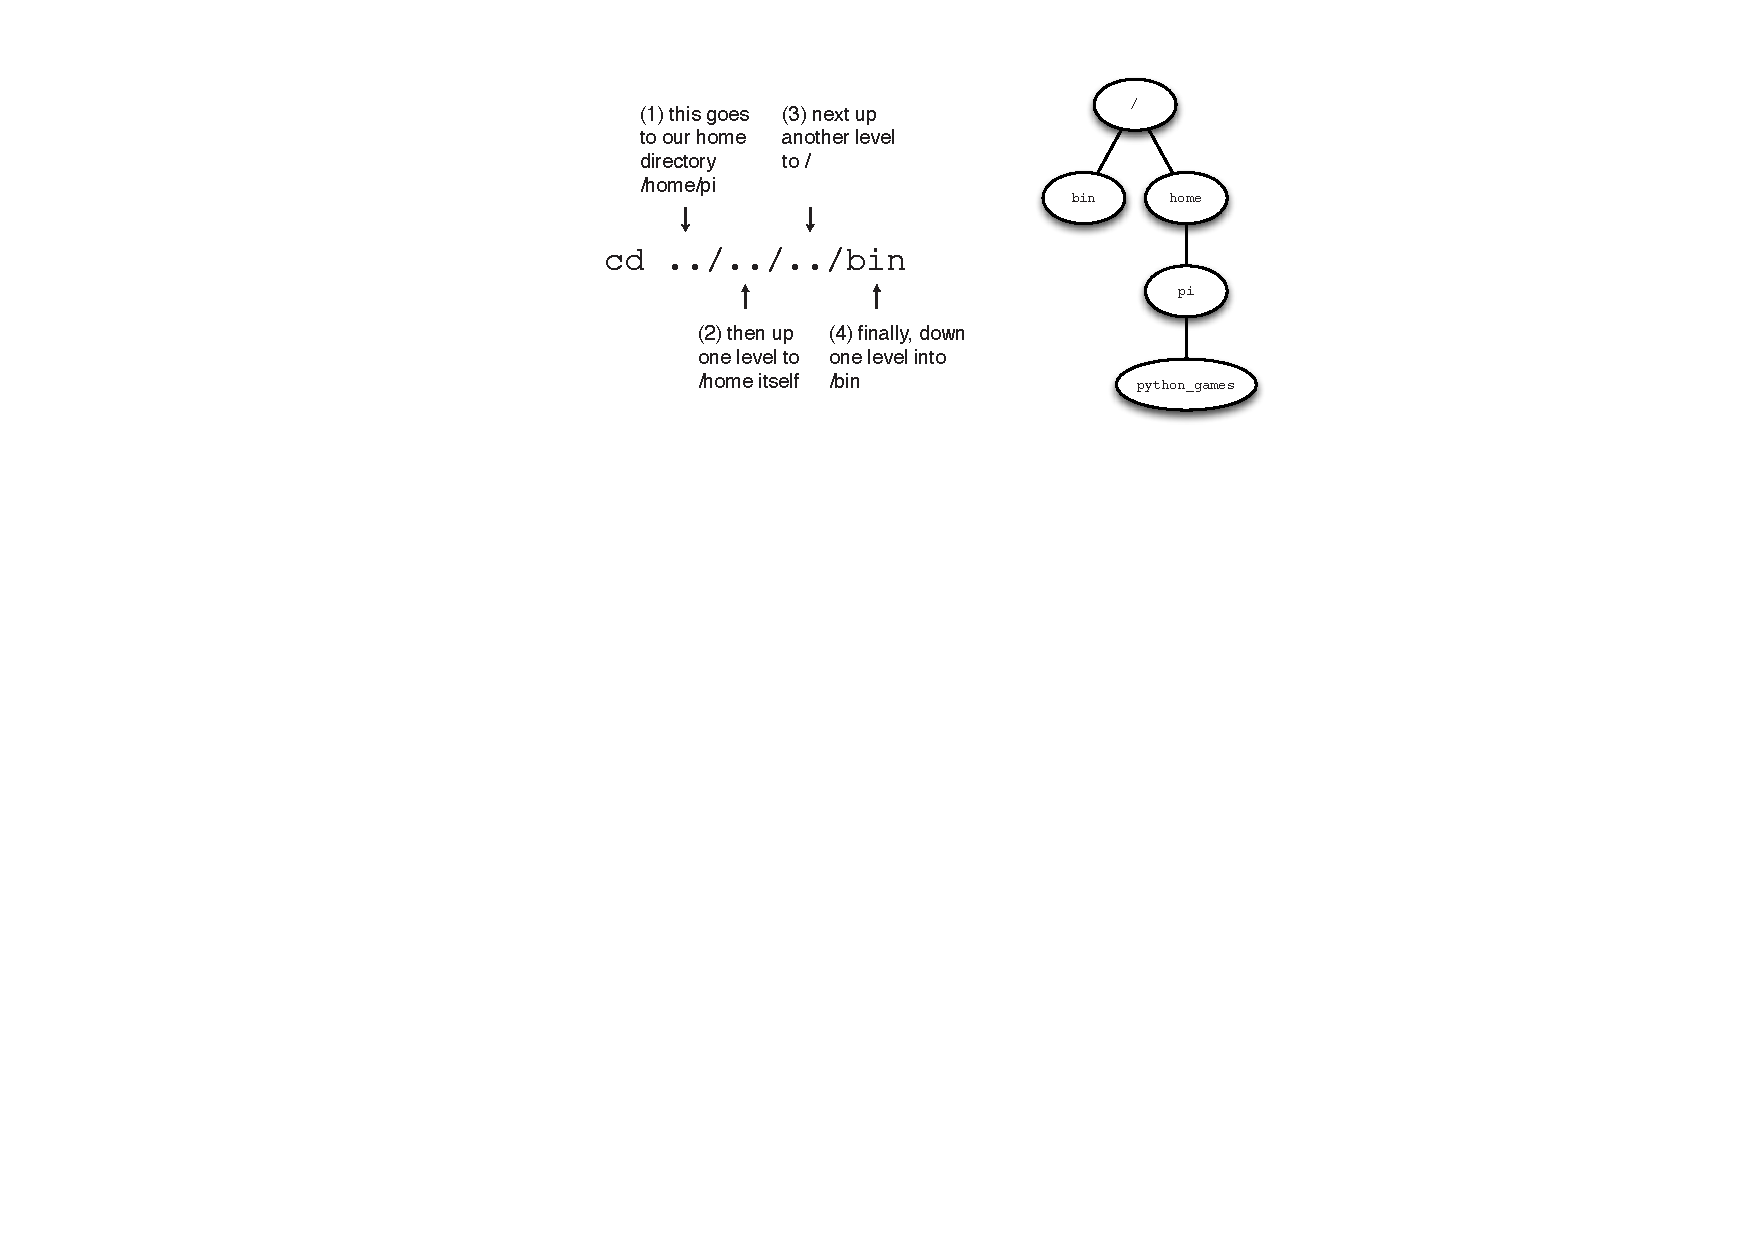
\includegraphics[width=13.5cm]{images/simple-navigation}}
\caption{Given the Pi's default filesystem structure, starting in the \fname{python\_games} directory, the command \cmnd{cd}{cd ../../../bin} will take you to the \fname{/bin} directory (by an admittedly tortuous route!)}\label{figure:simple-navigation}
\end{figure}

\subsection{Files in more detail}

The files we've looked at so far, and the behaviour of the commands we've used to manipulate them shouldn't feel too alien---we're just doing similar things on the command line to actions that you'll have performed using a graphical interface before. But the Unix take on files is rather more sophisticated than this, and to understand that, we'll need to think in a bit more detail about what a file actually is. When we think of an image or a music track as being stored `in a file', what do we actually mean? 

In abstract terms, a file is just a sequence of numbers, ultimately stored in binary on some storage device such as a hard drive. The right program can interpret these numbers, and turn them into pictures on screen, or sounds coming out of your speakers. The wrong program would be able to make no sense of a file at all; if you could `display' an audio track on screen, or `play' an image file as sound, it would just be a meaningless mess. So there's nothing very special about a file that makes its contents mean one thing or another; it's just up to a program to interpret what's in the file correctly. So what are the properties of a file? So far we've seen that files have a filename, and a location within a file system. We've seen that some files can be executed (which means their contents are instructions to the computer's CPU to do something), whereas other files contain data. But in both these cases, files are just sequences of numbers. Although we've not explored this yet, some files can be written to or modified, whereas others can only be read from; but they are still just sequences of numbers which when interpreted correctly have a particular meaning. 

The designers of Unix exploited this idea to create a very elegant way of representing the hardware of the underlying computer, and many of the properties of the operating system by treating anything that can be thought of as behaving like a file as being a file. 

What, for example, might a hard disk look like to the operating system? Well, a hard disk is a device that can store a long sequence of numbers, and if you interpret those numbers correctly, they can be made to represent a filesystem. So as far as Unix is concerned, a hard disk is a bit like a file that you can read from and write to. 

What about a process? Well that's a sequence of numbers in memory that happen to be instructions to the CPU to do useful things; so that's a file too (probably in this case a read-only file). 

What about a keyboard? Surely that's not a file? Actually it can be thought of as having some file-like properties; it's a stream of numbers that represent the keys pressed by the user, so it too is a sort-of read-only file. And the console? That too is file-like\ldots because it represents a sequence of numbers that can be interpreted as the output from various processes; so it's a bit like a write-only file. 

This may seem all a bit esoteric and confusing right now, but as we explore more examples of these file-like things, you'll start to see how elegant the idea is. 

For now, to give this stuff about files some time to sink in a bit, let's play another game. 

\FloatBarrier
\section{The Colossal Cave}

We're now going to explore a bit of computing history, and install and play one of the very early computer games. Colossal Cave Adventure was the first `adventure game', in which a virtual world is described using only text, and the player controls the game's protagonist using simple textual commands. The game was created in 1976 by a keen caver called \wikipedia{William_Crowther}{Will Crowther} who at time was a programmer at Bold, Berenek \& Newman, the company that developed \wikipedia{ARPANET}{ARPANET}, the forerunner to the modern Internet. He later collaborated with \wikipedia{Don_Woods_(programmer)}{Don Woods}, then a graduate student at Stanford University, to create the Colossal Cave Adventure as we would recognise it today. The original version consisted of around 700 lines of the \wikipedia{Fortran}{FORTRAN} programming language and a similar number of lines of data. When running on a \wikipedia{PDP-10}{PDP-10} (see Figure~\ref{figure:cern-pdp-10} for a picture of what one of these machines looked like) Colossal Cave would consume around half of the machine's memory. To put this in perspective, the tiny Raspberry Pi computer on your desk has roughly 1000 times as much memory as the PDP-10; it can run Colossal Cave with ease. 

\begin{figure}[t]
\centerline{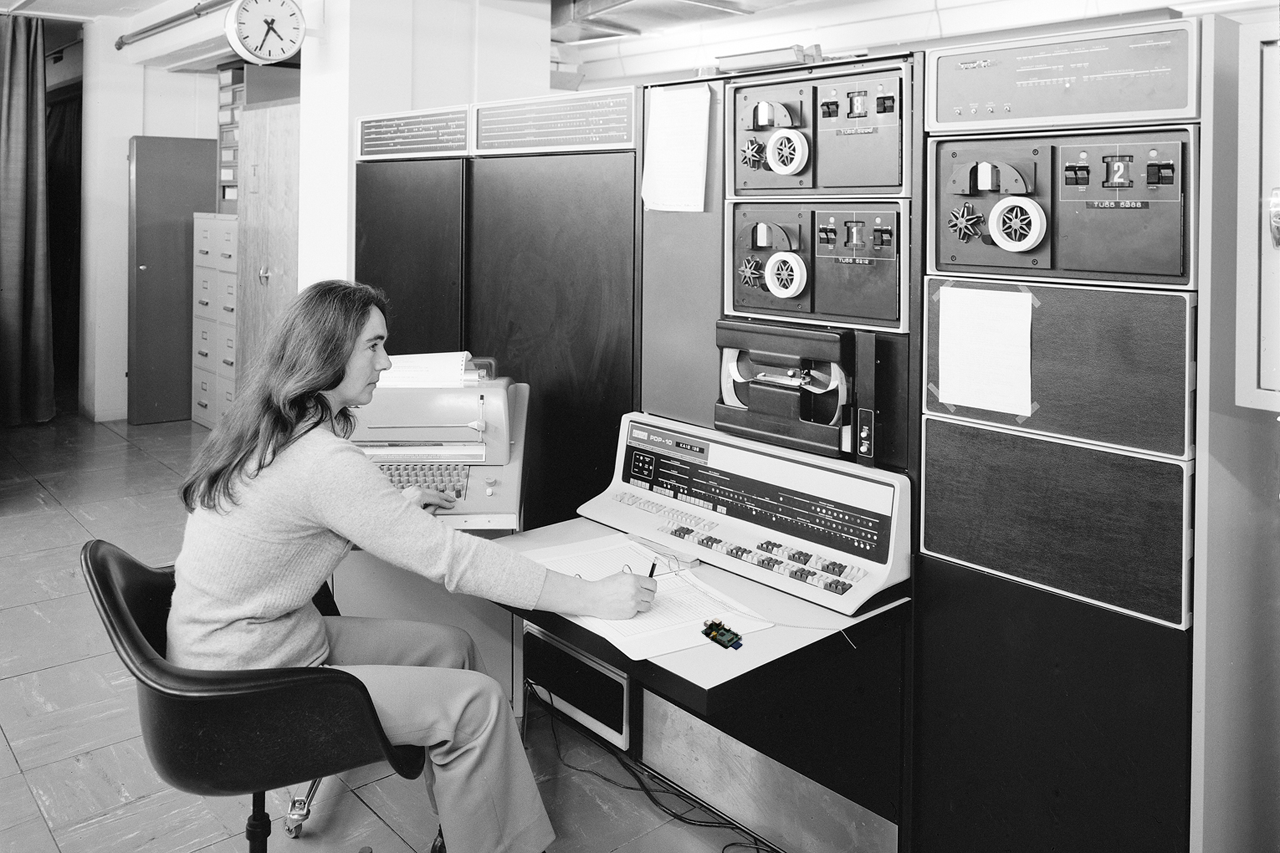
\includegraphics[width=14cm]{images/cern-pdp10+pi.png}}
\caption{A PDP-10 from CERN, circa 1974, reproduced with permission. \urlnop{cds.cern.ch/record/916840}. We've taken the liberty of crudely superimposing a Raspberry Pi to approximately the right scale on the operator's desk, just to give a sense of the difference in size between the two machines.}\label{figure:cern-pdp-10}
\end{figure}

Although the original FORTRAN source code for Colossal Cave still exists, the version you're going to play with is based on a re-implementation of the game on what became known as the \wikipedia{Z-machine}{Z-Machine}: a \wikipedia{Virtual_Machine}{virtual machine} specifically for running interactive fiction games.\footnote{Don't confuse the Z-machine, which is a virtual machine for adventure games, with the Z Machine, which is the largest X-ray generator in the world. Doing so is likely to make your lamp melt, and the trolls very grumpy.}
 
\FloatBarrier
\subsection{Installing Frotz, a Z-Machine Interpreter}

Unlike the other commands that you've used so far, the program we need to be able to play Colossal Cave Adventure isn't pre-installed on the Raspberry Pi, so we're going to have to fetch and install it ourselves. Fortunately, the version of Linux that we have on the Pi comes with a package management system that makes this quite easy. 

But first, we're going to have to understand a command called \cmnd{sudo}{sudo}. Everything that you've done so far has involved looking at files that either belong to the `pi' user, or are parts of the system that can be read or executed by any user. But of course, installing a new piece of software involves \textit{modifying} the Pi's operating system in some way, and that's not something that you want to do casually since mistakes could potentially mess up the whole device. 

You'll be familiar with the idea of a user with \wikipedia{Administrators}{Administrator privileges} from Windows or OS X; on Linux the \wikipedia{Superuser}{superuser} that can do anything to any part of the system is called `root' (because this user can modify any part of the system from the root of the filestore downwards). In the early days of Unix, administrators would log in as the root user to modify, update and repair the system. This had two major downsides: first, that if you accidentally left yourself logged in as the superuser when you nipped out for a coffee, the machine was vulnerable to misuse by anybody who would get at the keyboard; but second and more serious, all the normal safety nets that prevent you from accidentally deleting or damaging the operating system itself are deactivated, so its much easier for a slip of the finger or a brief moment of stupidity to have disastrous effects. To avoid these problems, Unix systems now usually recommend the use of the \cmnd{sudo}{sudo} ('Super User Do') command to temporarily elevate a normal user's privilege to that of super user for a single command. 

The system that we're going to use to install this game is called \cmnd{apt}{apt}, which stands for \wikipedia{Advanced_Packaging_Tool}{Advanced Packaging Tool}. This tool maintains a list of remote \textit{repositories} in which packages have been put that contain all the programs, libraries and data files necessary to install a particular Linux program. It can deal with fetching packages over the Internet, as well as extracting and copying their contents into the right places on your system. It also performs a series of sanity-checks to make sure that what you're adding is compatible with whatever you've already got in place.

The system we want to install to play this game is called \ttout{frotz} (to learn why, you'll have to play the game a bit, or look it up on Google) Let's try running the \cmnd{apt-get}{apt-get} command \textit{without} having gained superuser privilege first. Try typing:

\begin{ttoutenv}
$ apt-get install frotz
\end{ttoutenv}

\noindent The operating system will respond with something like:

\begin{alltt}
  \small
E: Could not open lock file /var/lib/dpkg/lock - open (13: Permission denied)
E: Unable to lock the administration directory (/var/lib/dpkg/), are you root?
\end{alltt}

Notice the question at the end: `are you root?'. Well, no you're not, so Linux has rightly prevented you from performing this operation. Now we'll try again using the \totype{sudo} command. This time type:

\begin{ttoutenv}
$ sudo apt-get install frotz
\end{ttoutenv}

You should see a series of lines printed out on the console, ending with:

\begin{ttoutenv}
Setting up frotz (2.43-4) ...
\end{ttoutenv}

\noindent before being returned to the command prompt (note the version number for frotz may have changed from 2.43-4 by the time you do this exercise, don't worry, that's fine). It's possible that \cmnd{apt-get}{apt-get} will fail to find the frotz package in one of the repositories it knows about; if this happens, it's usually because the repository has moved somewhere else on the internet, so you need to tell the APT system to update itself first: run the command \ttout{sudo apt-get update}, and when that has completed try installing the frotz package again, and all should be well. 

\begin{rpi}{APT}
The APT system is a very convenient way of managing packages, since it will automate the process of finding, fetching, configuring and installing software on your Pi (or indeed, on other Debian-based Linux installations). The RPM system does something similar for distributions based on Red Hat's version of Linux.

The various repositories that contain the packages for your Pi are updated regularly, so it's worth running \cmnd{apt-get}{apt-get update} once in a while to refresh your Pi's list of software. 

You should also at some point run \cmnd{apt-get}{apt-get upgrade}, which will cause all the packages that have already been installed to be upgraded to the latest version that the APT system can find. This lab will work just fine with the versions of software that are pre-installed on your Pi, and the upgrade process can take quite some time (hours, possibly), so you mustn't do it now or you won't be able to complete this lab in time. Try it at home, or outside of a lab session. 
\end{rpi}

The \ttout{frotz} system on its own is just a virtual machine into which you can load adventure game data, so we'll need to fetch the Colossal Cave datafile before we can play anything. We've put a copy of the game on the web at:

\noindent \urlnop{studentnet.cs.manchester.ac.uk/ugt/COMP10120/files/Advent.z5} 

\noindent so you can fetch it from there. Oh, hang on. No web browser. Oh dear.

Although it is actually possible to browse the web in console mode on the Pi (we'll experiment in another lab session because there are interesting lessons to be learned by doing so), there's an easier way to interact with the web to get the file that we need, using a command called \cmnd{curl}{curl}. First, use \cmnd{cd}{cd} to change to your home directory if you're not there already, then

\begin{ttoutenv}
\footnotesize
$ curl http://studentnet.cs.manchester.ac.uk/ugt/COMP10120/files/Advent.z5 -o Advent.z5
\end{ttoutenv} 

\noindent and you'll see \totype{curl} fetch the file you need `over the web' and save it in your home directory. This is also the first time you've encountered what's called a command-line argument \concept{switch}: the \ttout{-o} switch tells \cmnd{curl}{curl} to use the next argument on the command line as the output filename. 

Use \cmnd{ls}{ls} to confirm that you can see the file \fname{Advent.z5} in your home directory, then type: 

\begin{ttoutenv}
$ frotz Advent.z5
\end{ttoutenv}

\noindent to start playing the Colossal Cave Adventure. Once the game has started (the screen will have gone blue), type HELP to get instructions. When you've had a bit of a wander around and got the general idea of the game, you can type quit to get back to the command prompt. There are some parallels between using commands to wander around Colossal Cave and using Unix commands to navigate around the Pi's filesystem. There's a map of the entire Colossal Cave world in Appendix \ref{appendix:colossal-map}, and we'll look at some commands that will help you if you get totally lost in a Unix filesystem in %section \ref{section:advanced-navigation} in
a later lab session.

Earlier, we referred to Colossal Cave as a work of Interactive Fiction (IF). In truth, this is perhaps stretching the term somewhat, since the genre has matured considerably in the decades since this first adventure game. For a much more compelling example of Interactive Fiction with beautifully written prose, and funny and challenging puzzles we suggest you have a go at playing Curses by \wikipedia{Graham_Nelson}{Graham Nelson}, or one of the many other games written by Interactive Fiction enthusiasts that are available for free from \url{www.ifarchive.org}. If you find yourself getting hooked on playing IF, the frotz interpreter is available for most platforms, including iOS, Android, OS X and Windows. 

\section{Quake}

We'll finish this lab session off with one more game. 

Use \cmnd{curl}{curl} to fetch the file hosted at
\\
\urlnop{studentnet.cs.manchester.ac.uk/ugt/COMP10120/files/quake3.tar.gz}
\\
making sure you save it in your home directory. 

Notice that this file ends with \fname{.tar.gz}. The \fname{.gz} suffix tells us that this file has been compressed using a utility called \cmnd{gzip}{gzip}, so the first task is to uncompress the file. Type:

\begin{ttoutenv}
$ gunzip quake3.tar.gz
\end{ttoutenv}

This will uncompress the file, removing the \fname{.gz} and leaving you with \fname{quake3.tar}. A `tarfile' a bundle of individual files that have been assembled together into a single file for convenience (you'll probably have already encountered `zip' files, which have a similar purpose). The name `tar' is an abbreviation of 'Tape Archive', since the \cmnd{tar}{tar} command was originally used for making backups of filestores onto tape. It remains, however, a very versatile way of bundling up lots of things, and you'll find \cmnd{tar}{tar} files all over the internet. 

To see what's in this archive, run the command 

\begin{ttoutenv}
$ tar tf quake3.tar
\end{ttoutenv}

\noindent and you'll see a long list of the archive's contents scroll past on the screen. The first argument to \cmnd{tar}{tar} is a bit of an odd one, since it's a collection of options, which unusually for Unix are not prefixed by individual minus signs (recall the \ttout{-o} option we used for \totype{curl}; that's a far more common way of specifying options to tools). In this case the options mean:

\begin{itemize}
\item the \textbf{t} causes \totype{tar} to list the `table of contents', for the archive, without extracting anything.
\item the \textbf{f} tells tar that the next argument is the file containing the archive. 
\end{itemize}

\noindent To actually extract the contents of the archive we issue the command:

\begin{ttoutenv}
$ tar xvf quake3.tar
\end{ttoutenv}

\noindent where

\begin{itemize}
\item \textbf{x} means `extract'.
\item \textbf{v} means `be verbose, and show what you're extracting as you do it'.
\item \textbf{f} again means `and here is the file to work on'.
\end{itemize}

\noindent When tar has finished working you're presented again with the command prompt. Use \cmnd{ls}{ls} to confirm that you now have a directory called \fname{quake3} in your home directory.  You might also want to plug some headphones into the Pi at this point too, if you happen to have a pair with you. 

\begin{ttoutenv}
$ cd quake3
$ ./ioquake3.arm
\end{ttoutenv}

\noindent After the startup screen, the game will ask you for a code, but you can just skip this and use the mouse to select the play option. The rest, we're sure, you can figure out for yourself. 

\begin{diversion}{Multiplayer Quake?}
You can play this version of Quake3 Arena with friends over the network. We'll leave you to figure out how to configure that yourself (hint: the \cmnd{ifconfig}{ifconfig} command will tell you what IP address has been allocated to your Pi).
\end{diversion}

\FloatBarrier
\section{RTFM}

Although we've introduced several Unix commands in this lab, we've only done so quite superficially today, giving you just enough detail to get through the tasks in this tutorial. Each of the commands is much more powerful than what you've been exposed to so far. Though you won't need to know every possible option off by heart, there are a lot of useful things you can learn about them quite easily. 

Most Unix systems, including the one on your Pi have an instruction-manual system that gives more details about the available commands (and most things that you install yourself, such as \totype{frotz} also install their own manual pages).  Try running:

\begin{ttoutenv}
$ man ls
\end{ttoutenv}

\noindent for information on the \totype{ls} command, and use the same trick to find out more about the other commands you've seen today. If you need more help on how to use the \cmnd{man}{man} command, you can always use: 

\begin{ttoutenv}
$ man man
\end{ttoutenv}

\noindent When you're looking at a manual page, pressing the Space Bar will advance you on a page, and the Up and Down cursor keys will move you back and forth line-by-line. Press `q' to quit viewing a man page. 

\begin{diversion}{RTFM?}
The acronym RTFM stands for Read The Flipping Manual, and is sometimes used as a response when somebody has asked a lazy question on a forum or by email where decent documentation already exists and is easily accessible. The F is usually interpreted as meaning something less polite than `Flipping'. 
\end{diversion}

\FloatBarrier
\section{Shutting down your Pi safely}
\label{section:shutdown}

When you're finished playing Quake, exit the game and get back to the command prompt. Like any other computer, its really important that you shut your Pi down properly; if you just pull the power cord out there's a chance of corrupting the filesystem. To shut the Pi down safely using the \cmnd{halt}{halt} command:

\begin{ttoutenv}
$ sudo halt
\end{ttoutenv}

\noindent You'll see the a series of messages scroll past that look rather like those you saw during the boot process. This shouldn't be surprising, since what the operating system is doing now is shutting down all the things that it started up when you booted the machine, roughly in reverse order. When all these services have closed down tidily, the Pi will power itself down; the network  and OK LEDs will go off, the screen should go black, and only the red PWD LED will remain lit on the circuit board. At this point its safe to pull the Micro-USB cable out of the Pi. 

\FloatBarrier
\section{What have you learned?}

It might seem like you've been playing games for most of the lab, but if you've followed the instructions carefully and read through all the text you'll have learned a lot of new things. These include:
\begin{itemize}
\item the anatomy of a pi
\item how to safely start and stop your Pi
\item running commands: \totype{tar}, \totype{cd}, \totype{ls}, \totype{pwd}, \totype{unzip}, \totype{sudo}
\item how the filestore is structured
\item basic apt commands
\end{itemize}




%\printbibliography

